O Selection Sort é outro algoritmo de ordenação simples e intuitivo. Ele divide a lista de entrada em duas partes: a sublista de itens já ordenados e a sublista de itens ainda a serem ordenados. Em cada iteração, o algoritmo procura o menor (ou maior, dependendo da ordem desejada) elemento da sublista não ordenada e o troca com o primeiro elemento da sublista não ordenada. Este processo é repetido até que toda a lista esteja ordenada. Apesar de sua simplicidade, o Selection Sort pode ser ineficiente para listas muito grandes.

 \begin{figure}[h!]
    \centering
    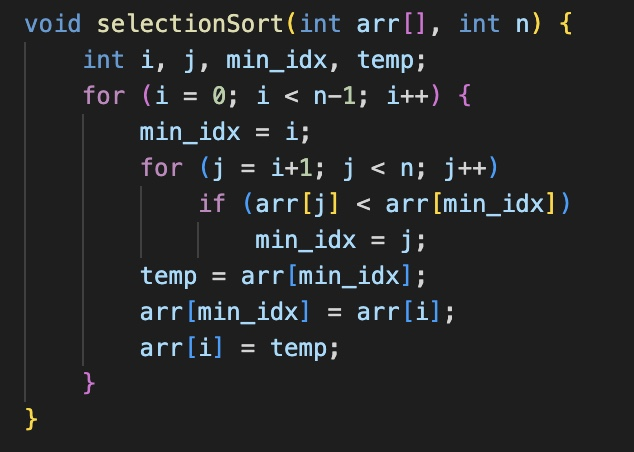
\includegraphics[width = 10cm]{Imagens/Selection Sort/Imagemselection.jpg}
    \caption{ALgoritmo Selection Sort, imagem criada pelo autor. }
    \label{imagem_insert}
\end{figure}

Exemplo: 

Vamos considerar o seguinte array como exemplo \cite{site2023}: arr[]= {64, 25, 12, 22, 11}
\par Primeiro passo conforme à figura \ref{fig:enter-label}: para a primeira posição na matriz, toda a matriz é percorrida do índice 0 ao 4, subsequencialmente. A primeira posição onde 64 está armazenado atualmente, depois de percorrer todo o array, chega a conclusão de que o 11 é o menor valor. Assim, substitua o 64 por 1. Após uma iteração, 11, que é o menor valor da matriz, passa a aparecer na primeira posição da lista ordenada. 

\begin{figure} [h!]
    \centering
    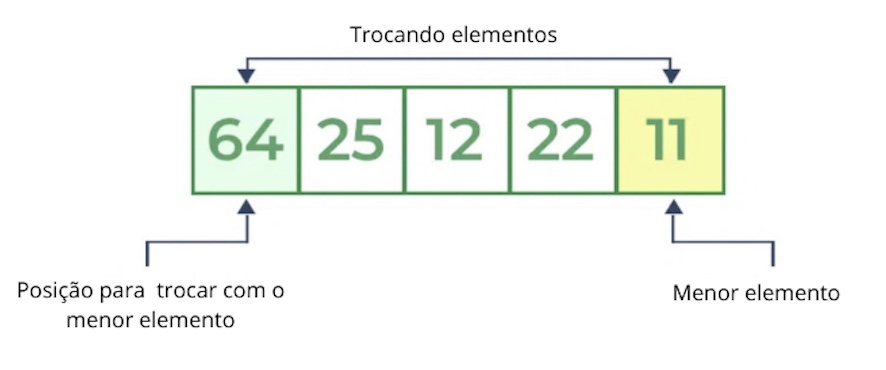
\includegraphics[width = 10cm]{Imagens/Selection Sort/Imagem 27-09-2023 às 16.06.jpeg}
    \caption{Selection Sort | Trocando o 1º elemento pelo mínimo do array}
    \label{fig:enter-label}
\end{figure}

\par Segundo passo conforme à figura \ref{fig:exemplo2}: para a segunda opção, onde o 25 está ocupando, percorra novamente todo o array. Após percorrer, descobrimos que 12 é o segundo menor valor do array e deve aparecer na segunda opção, portanto realiza a troca desses valores.

\begin{figure}[h!]
    \centering
    \includegraphics[width = 10cm]{Imagens/Selection Sort/Captura de Tela 2023-09-27 às 16.15.34.png}
    \caption{Selection Sort | trocando i=1 pelo próximo elemento mínimo}
    \label{fig:exemplo2}
\end{figure}
\newpage
\par Terceiro passo conforme à figura \ref{fig:exemplo3}: agora, para o terceiro lugar, onde 25 está presente, percorra novamente o restante do array e encontre o terceiro menor valor presente no array. Durante o processo, 22 acabou sendo o terceiro menor valor e deveria aparecer na terceira posição do array, portantanto troque 22 pelo elemento presente na terceira posição.

\begin{figure}[h!]
    \centering
    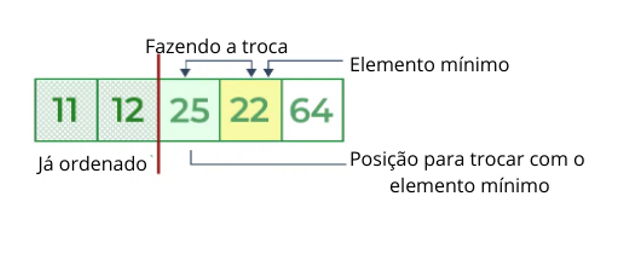
\includegraphics[width = 10cm]{Imagens/Selection Sort/image1.png}
    \caption{Selection Sort | trocando i=2 pelo próximo elemento mínimo}
    \label{fig:exemplo3}
\end{figure}

\par Quarto passo conforme à figura \ref{fig:exemplo4}: da mesma forma que os anteriores, percorra o resto da matriz e encontre o quarto menor elemento da matriz. Como 25 é o quarto valor mais baixo, ele ficará na mesma posição.

\begin{figure}[h!]
    \centering
    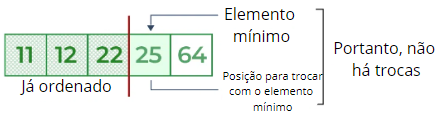
\includegraphics[width = 10cm]{Imagens/Selection Sort/image2.png}
    \caption{Selection Sort | trocando i=3 pelo próximo elemento mínim}
    \label{fig:exemplo4}
\end{figure}

\par Quinto passo conforma à figura \ref{fig:exemplo5}: por fim, o maior valor presente no arrray é automaticamente colocado na última posição do array, a matriz resultante é a matriz ordenada.

\begin{figure}[h!]
    \centering
    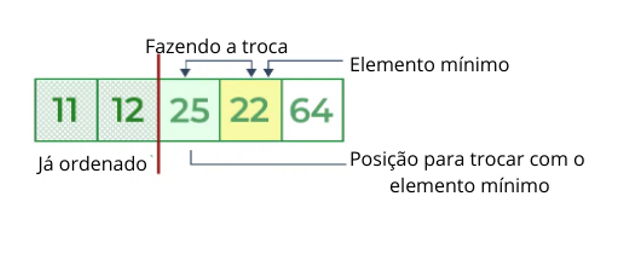
\includegraphics[width = 10cm]{Imagens/Selection Sort/image1.png}
    \caption{Selection Sort | Matriz ordenada}
    \label{fig:exemplo5}
\end{figure}